\documentclass[12pt,a4paper]{article}

%% ── Packages ─────────────────────────────────────────────────────────────────
\usepackage[margin=1in]{geometry}
\usepackage{graphicx}
\usepackage{amsmath}
\usepackage{hyperref}
\usepackage{booktabs}
\usepackage{array}
\usepackage{titlesec}
\usepackage{fancyhdr}
\usepackage{setspace}
\usepackage{enumitem}
\usepackage{listings}
\usepackage{xcolor}
\usepackage{float}
\usepackage{caption}
\usepackage{tikz}
\usetikzlibrary{shapes.geometric, arrows, positioning}

%% ── Header / Footer ──────────────────────────────────────────────────────────
\pagestyle{fancy}
\fancyhf{}
\lhead{\small CSE 4224 – Digital System Design Laboratory \hfill KUET}
\rfoot{\thepage}

%% ── Hyperref setup ───────────────────────────────────────────────────────────
\hypersetup{colorlinks=true, linkcolor=blue, urlcolor=blue}

%% ─────────────────────────────────────────────────────────────────────────────
\begin{document}

%% ── Title Page ───────────────────────────────────────────────────────────────
\begin{titlepage}
  \centering
  \vspace*{1.5cm}
  {\LARGE \textbf{KHULNA UNIVERSITY OF ENGINEERING \& TECHNOLOGY}}\\[0.8cm]
  \rule{\linewidth}{0.5pt}\\[0.4cm]
  {\large Course No: CSE 4224}\\[0.2cm]
  {\large Course Title: Digital System Design Laboratory}\\[0.4cm]
  \rule{\linewidth}{0.5pt}\\[1.5cm]
  {\huge \textbf{Frequency-Based Fixed Huffman Encoder}}\\[0.4cm]
  {\Large \textit{FPGA Deployment on Basys3 (Artix-7 XC7A35T)}}\\[2cm]
  {\large \textbf{Submitted By}}\\[0.6cm]
  \begin{tabular}{ll}
    \textbf{Md. Tanjimul Hasan}           & Roll No: 2007081 \\[0.3cm]
    \textbf{Md. Abu Loman Hossain Shuvo}  & Roll No: 2007073 \\
  \end{tabular}\\[2cm]
  {\large Department of Computer Science and Engineering}\\[0.3cm]
  {\large Khulna University of Engineering \& Technology}\\[0.3cm]
  {\large Khulna--9203, Bangladesh}\\[1.5cm]
  {\large April, 2026}
\end{titlepage}

%% ── Table of Contents ────────────────────────────────────────────────────────
\tableofcontents
\newpage

%% ─────────────────────────────────────────────────────────────────────────────
\section{Introduction}

\subsection{Background}
Data compression is a critical operation in modern digital systems to optimise storage and
transmission bandwidth. Huffman encoding is a widely adopted lossless data compression
algorithm that operates on the principle of variable-length symbol encoding: symbols
appearing most frequently are assigned the shortest binary sequences. In embedded systems
and telecommunications, executing these algorithms rapidly and deterministically is
paramount. FPGA-based implementations provide hardware-level parallelism, guaranteeing
deterministic, high-speed execution required for real-time compression—far surpassing the
throughput of equivalent software implementations on microcontrollers.

This updated project extends the original simulation-only Huffman encoder to a
\textbf{fully deployable hardware system} targeting the \textbf{Digilent Basys3 board}
(Artix-7 XC7A35T-1CPG236). Every design decision, from the choice of sorting algorithm
to the physical I/O mapping, is driven by the constraints and capabilities of real FPGA
hardware.

\subsection{Motivation}
The original design employed a combinational parallel comparator to assign ranks without
explicit sorting, which, while efficient in simulation, produced incorrect results when
equal-frequency symbols were present under real-world FPGA synthesis constraints.
Furthermore, the original 2-bit symbol bus and 16-word RAM were insufficient for
meaningful ASCII input from physical switches.

This iteration addresses all limitations:
\begin{itemize}
  \item Replaces the parallel comparator with a \textbf{hardware bubble sort} that
        correctly handles tie-breaking by frequency-sorted character index.
  \item Expands the symbol width to \textbf{8-bit ASCII} and the memory to a
        \textbf{128-word} RAM to support realistic switch-based input.
  \item Adds a fully wired \textbf{seven-segment display} for real-time interactive
        output, replacing the LED single-bit serial output.
  \item Implements \textbf{button debouncing and edge detection} to ensure glitch-free
        physical button operation at the 100\,MHz system clock.
\end{itemize}

%% ─────────────────────────────────────────────────────────────────────────────
\section{Objectives}

\subsection{Primary Objective}
To design, implement, synthesise, and physically deploy a hardware-based variable-length
frequency Huffman encoder on the Basys3 FPGA board using a Moore Finite State Machine
(FSM) architecture, with complete seven-segment interactive I/O.

\subsection{Specific Objectives}
\begin{enumerate}
  \item Develop a Moore FSM with \textbf{31 states} orchestrating the full encode pipeline:
        input capture, memory initialisation, bubble sort, rank fetch, and serial output.
  \item Design a \textbf{hardware bubble-sort} sub-routine that correctly sorts up to four
        symbol frequencies in descending order, with stable tie-breaking.
  \item Implement a \textbf{128-deep $\times$ 8-bit synchronous RAM} serving as both the
        input sequence buffer and the sort working space.
  \item Implement a \textbf{shift-register with dynamic bit-counter} to construct a
        variable-length serial data stream for each encoded symbol.
  \item Design a \textbf{four-digit seven-segment display controller} with hardware
        time-multiplexing to show the registered symbol and its Huffman code
        simultaneously on separate digits.
  \item Implement three-stage flip-flop synchronisers and rising-edge detectors on all
        four physical button inputs to eliminate metastability and contact bounce.
  \item Map all I/O signals to the correct Basys3 package pins via a Xilinx Design
        Constraints (\texttt{.xdc}) file and successfully generate the programming
        bitstream.
\end{enumerate}

%% ─────────────────────────────────────────────────────────────────────────────
\section{System Architecture}

The updated system architecture comprises \textbf{nine Verilog modules} connected
hierarchically under \texttt{top\_module}. It is divided into four functional
subsystems: the Control Unit FSM, the Memory Buffer, the Sorting and Frequency
Datapath, and the Display Subsystem.

\vspace{0.5cm}
\noindent\textit{Figure 1 shows the high-level block diagram of the system.}
\vspace{0.3cm}

\begin{figure}[H]
\centering
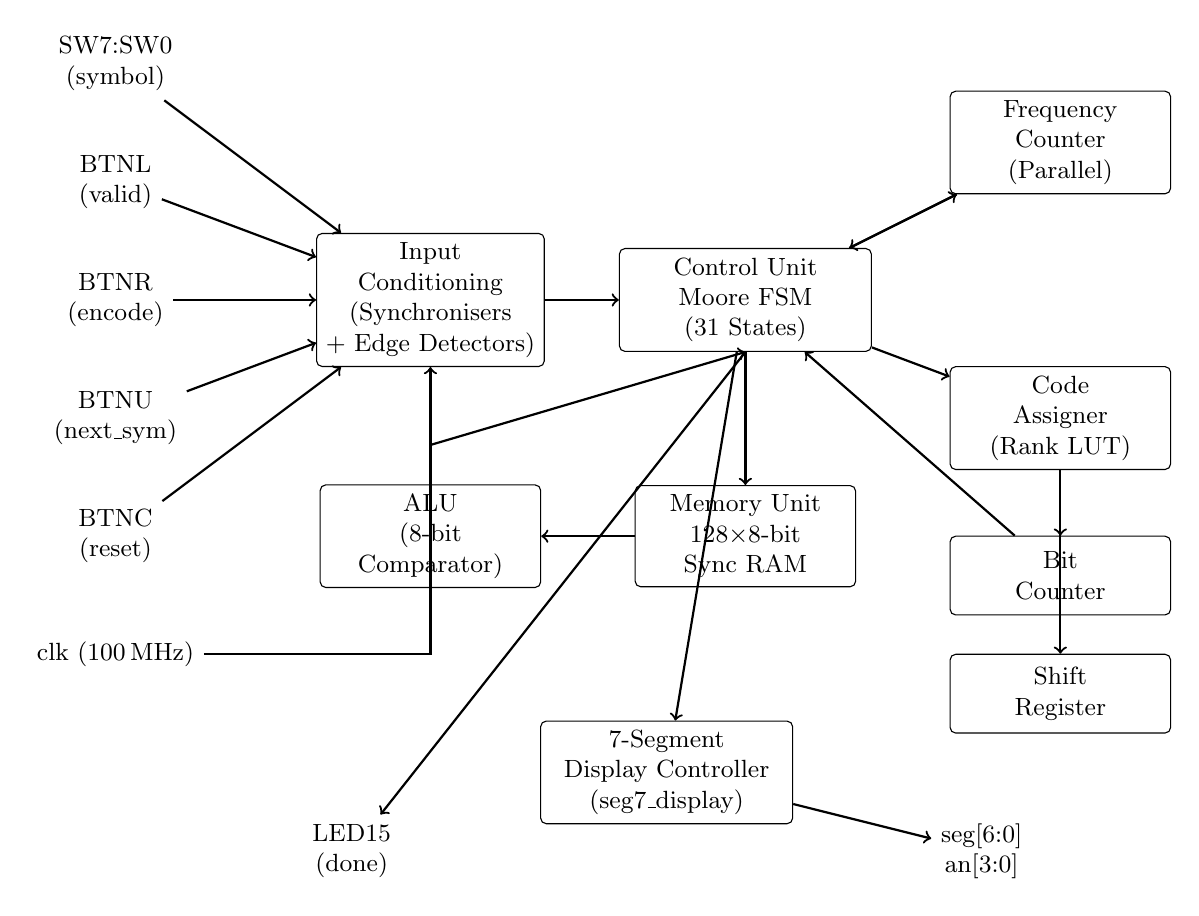
\begin{tikzpicture}[
  every node/.style={font=\small},
  block/.style={draw, rectangle, minimum width=2.8cm, minimum height=1cm,
                align=center, rounded corners=2pt},
  arrow/.style={->, thick}
]
  % Inputs
  \node[align=center] (sw)   at (0, 4)   {SW7:SW0\\(symbol)};
  \node[align=center] (btnl) at (0, 2.5) {BTNL\\(valid)};
  \node[align=center] (btnr) at (0, 1)   {BTNR\\(encode)};
  \node[align=center] (btnu) at (0,-0.5) {BTNU\\(next\_sym)};
  \node[align=center] (btnc) at (0,-2)   {BTNC\\(reset)};
  \node[align=center] (clk)  at (0,-3.5) {clk (100\,MHz)};

  % Input conditioning block
  \node[block] (cond) at (4, 1) {Input\\Conditioning\\(Synchronisers\\+ Edge Detectors)};

  % Control Unit
  \node[block, minimum width=3.2cm] (cu) at (8, 1) {Control Unit\\Moore FSM\\(31 States)};

  % Memory
  \node[block] (mem) at (8, -2) {Memory Unit\\128$\times$8-bit\\Sync RAM};

  % ALU
  \node[block] (alu) at (4, -2) {ALU\\(8-bit\\Comparator)};

  % Freq counter
  \node[block] (fc)  at (12, 3) {Frequency\\Counter\\(Parallel)};

  % Code assigner
  \node[block] (ca)  at (12,-0.5) {Code\\Assigner\\(Rank LUT)};

  % Bit counter
  \node[block] (bc)  at (12,-2.5) {Bit\\Counter};

  % Shift register
  \node[block] (sr)  at (12,-4) {Shift\\Register};

  % Display
  \node[block, minimum width=3.2cm] (disp) at (7, -5) {7-Segment\\Display Controller\\(seg7\_display)};

  % Outputs
  \node[align=center] (seg) at (11,-6) {seg[6:0]\\an[3:0]};
  \node[align=center] (led) at (3, -6) {LED15\\(done)};

  % Arrows
  \draw[arrow] (sw) -- (cond);
  \draw[arrow] (btnl) -- (cond);
  \draw[arrow] (btnr) -- (cond);
  \draw[arrow] (btnu) -- (cond);
  \draw[arrow] (btnc) -- (cond);
  \draw[arrow] (clk) -| (cond);
  \draw[arrow] (cond) -- (cu);
  \draw[arrow] (cu) -- (mem);
  \draw[arrow] (cu) -- (ca);
  \draw[arrow] (mem) -- (alu);
  \draw[arrow] (alu.north) -- ++(0,0.5) -- (cu.south);
  \draw[arrow] (ca) -- (bc);
  \draw[arrow] (ca) -- (sr);
  \draw[arrow] (bc) -- (cu);
  \draw[arrow] (cu) -- (fc);
  \draw[arrow] (fc) -- (cu);
  \draw[arrow] (cu) -- (disp);
  \draw[arrow] (disp) -- (seg);
  \draw[arrow] (cu.south) -- (led);
\end{tikzpicture}
\caption{System Architecture of the Updated Huffman Encoder (Basys3 Deployment)}
\end{figure}

\subsection{Control Unit}
The control unit is the central orchestrator. Implemented as a Moore FSM with
\textbf{31 states}, it generates all synchronisation signals: RAM write-enable, address,
and data buses; ALU operand latching triggers; load and shift enables for the output
datapath; and digit-latching pulses for the display controller. All outputs are registered
with explicit reset values to prevent Vivado synthesis warnings.

\subsection{Memory Buffer}
A \textbf{128-word $\times$ 8-bit} single-port synchronous RAM serves dual purposes.
Addresses 0--3 store the four symbol frequencies; addresses 4--7 store the corresponding
ASCII characters for sort co-movement; addresses 8--127 store the chronological input
sequence entered by the user via the DIP switches. Independent 7-bit write and read
pointers manage the input buffer, both initialised to address 8 on reset.

\subsection{Sorting Datapath}
Rather than parallel combinational comparators, the updated design implements a
\textbf{hardware bubble sort} sub-routine fully sequenced by the FSM.
An 8-bit ALU (\texttt{alu.v}) provides the less-than comparison used in the sort logic.
Two 8-bit staging registers (\texttt{reg\_f\_a}, \texttt{reg\_f\_b}) hold frequency
values read in consecutive cycles before comparison. A symmetric pair
(\texttt{reg\_c\_a}, \texttt{reg\_c\_b}) holds the corresponding character values during
swap operations, ensuring co-movement of frequency and character arrays.

\subsection{Frequency Counter}
The \texttt{frequency\_counter} module maintains four independent 8-bit saturating
accumulators, one per symbol (A, B, C, D). On every rising edge where
\texttt{count\_enable} is high, the accumulator whose ASCII address matches the incoming
\texttt{symbol[7:0]} is incremented. The four frequency values are available as parallel
8-bit outputs directly consumed by the FSM during the memory initialisation phase.

\subsection{Output Datapath}
The output datapath is composed of:
\begin{itemize}
  \item \textbf{Code Assigner} (\texttt{code\_assigner.v}): A 4-entry rank-to-code
        lookup table mapping rank $\in \{1,2,3,4\}$ to a 3-bit code and 2-bit length.
  \item \textbf{Shift Register} (\texttt{shift\_register.v}): A 3-bit parallel-load,
        left-shift register exposing the MSB as \texttt{serial\_out}.
  \item \textbf{Bit Counter} (\texttt{bit\_counter.v}): A down-counter loaded with
        the code length; asserts \texttt{zero\_flag} when the full code has been shifted,
        triggering a FSM state transition.
\end{itemize}

\subsection{Seven-Segment Display Controller}
The \texttt{seg7\_display} module drives the Basys3 four-digit common-anode
seven-segment display. It performs hardware time-multiplexing at approximately
$191\,\text{Hz}$ per digit using a 17-bit refresh counter clocked at 100\,MHz.
Two independent latching mechanisms are implemented:
\begin{itemize}
  \item \textbf{Symbol latch}: captures the 8-bit ASCII value on each \texttt{valid\_pulse},
        decodes it to the corresponding segment pattern (A, b, C, d), and holds it on
        digit AN3 (leftmost).
  \item \textbf{Code latch}: captures \texttt{huff\_code[2:0]} and
        \texttt{huff\_len[1:0]} on each \texttt{load\_pulse} (one cycle per encoded
        symbol) and decodes the individual bits as `0', `1', or `--' across digits
        AN2--AN0.
\end{itemize}

\subsection{Input Conditioning}
All four button inputs are passed through a \textbf{three-stage flip-flop synchroniser}
followed by a \textbf{rising-edge detector}, producing a single-cycle pulse per button
press irrespective of how long the button is held. This eliminates metastability,
eliminates contact bounce, and ensures each button press registers exactly one event
in the digital system.

%% ─────────────────────────────────────────────────────────────────────────────
\section{Finite State Machine Design}

The encoder controller is implemented as a Moore Finite State Machine. In a Moore FSM
the outputs depend solely on the current state, providing stable, glitch-free control
signals on every clock edge.

\subsection{FSM States}
The controller comprises \textbf{31 states} encoded in a 5-bit register, divided into
six operational phases:

\begin{table}[H]
\centering
\caption{FSM State Summary}
\begin{tabular}{lll}
\toprule
\textbf{Phase} & \textbf{States} & \textbf{Purpose} \\
\midrule
Input Capture   & \texttt{IDLE}, \texttt{COUNT}                                 & Accept symbols from BTNL        \\
Mem Init        & \texttt{MEM\_INIT\_F0--F3}, \texttt{MEM\_INIT\_C0--C3}        & Write freq \& ASCII to RAM      \\
Bubble Sort     & \texttt{SORT\_START} through \texttt{SORT\_NEXT\_J} (10 states) & Sort freq descending           \\
Rank Fetch      & \texttt{FETCH\_C1--C4}                                        & Read sorted chars into rank regs\\
Encode          & \texttt{ENCODE\_READ}, \texttt{ASSIGN}, \texttt{LOAD},        & Output Huffman codes serially   \\
                & \texttt{SHIFT}, \texttt{SHOW\_CODE}                           &                                 \\
Terminal        & \texttt{DONE}                                                 & Assert done, return to IDLE     \\
\bottomrule
\end{tabular}
\end{table}

\subsection{State Transition Logic}
Transitions are governed by both external button pulses and internal datapath flags:

\begin{itemize}
  \item \textbf{IDLE $\to$ COUNT}: Triggered by \texttt{valid\_pulse} (BTNL rising edge),
        the first symbol is written to RAM and the write pointer is incremented.
  \item \textbf{COUNT $\to$ MEM\_INIT\_F0}: Triggered by \texttt{encode\_pulse}
        (BTNR rising edge), decoupling symbol entry from encoding start.
  \item \textbf{Bubble Sort loop}: \texttt{SORT\_NEXT\_J} decrements the outer loop
        counter; when the inner loop is exhausted it either continues outer
        iterations or proceeds to \texttt{FETCH\_C1} once \texttt{sort\_i == 1}.
  \item \textbf{SHIFT $\to$ SHOW\_CODE}: When \texttt{zero\_flag = 1}, the FSM pauses;
        the display holds steady showing that symbol's code.
  \item \textbf{SHOW\_CODE $\to$ ENCODE\_READ}: Triggered by \texttt{next\_sym}
        (BTNU rising edge), advancing to the next input symbol.
  \item \textbf{ENCODE\_READ $\to$ DONE}: When the read pointer equals the write pointer,
        the entire sequence has been encoded; \texttt{done} is asserted for one cycle.
\end{itemize}

%% ─────────────────────────────────────────────────────────────────────────────
\section{Frequency Counting and Hardware Bubble Sort}

\subsection{Frequency Counting}
The \texttt{frequency\_counter} module accumulates symbol counts during the
\texttt{COUNT} phase. Each of the four accumulators is activated by comparing the
incoming \texttt{symbol[7:0]} against fixed ASCII values:

\begin{equation}
  f_k = \sum_{t=0}^{N-1} \mathbf{1}\!\left[\,\text{symbol}(t) = \text{ASCII}_k\,\right],
  \quad k \in \{A, B, C, D\}
\end{equation}

\subsection{Hardware Bubble Sort}
Unlike the original design's combinational ranking comparator, the updated system
implements a \textbf{multi-cycle hardware bubble sort} that physically reorders both
the frequency array (addresses 0--3) and the character array (addresses 4--7) inside the
RAM. The sort runs in descending frequency order with \textbf{strict greater-than
comparison} for tie-breaking: ties are \emph{not} swapped, so earlier-entered symbols
retain a higher rank. The sort complexity across outer/inner loop iterations is $O(n^2)$
in FSM states, with $n = 4$, requiring at most 24 comparison cycles before proceeding.

After sorting, the FETCH phase reads characters at addresses 4--7 (now sorted) into
rank registers \texttt{rank\_sym\_1}, \texttt{rank\_sym\_2}, \texttt{rank\_sym\_3}.
A combinational assignment then maps each \texttt{fetched\_symbol} to its rank:

\begin{equation}
  \texttt{current\_rank} =
  \begin{cases}
    1 & \text{if fetched\_symbol} = \texttt{rank\_sym\_1} \\
    2 & \text{if fetched\_symbol} = \texttt{rank\_sym\_2} \\
    3 & \text{if fetched\_symbol} = \texttt{rank\_sym\_3} \\
    4 & \text{otherwise}
  \end{cases}
\end{equation}

%% ─────────────────────────────────────────────────────────────────────────────
\section{Encoding Configuration}

Based on the rank computed from the sorted order, the \texttt{code\_assigner}
module translates the hierarchy into standard prefix-free variable-length binary codes.

\begin{table}[H]
\centering
\caption{Huffman Encoding Mapping by Rank}
\begin{tabular}{ccc}
\toprule
\textbf{Rank} & \textbf{Output Code} & \textbf{Bit Length} \\
\midrule
1 & \texttt{0}   & 1 \\
2 & \texttt{10}  & 2 \\
3 & \texttt{110} & 3 \\
4 & \texttt{111} & 3 \\
\bottomrule
\end{tabular}
\end{table}

Because the code length changes dynamically per symbol, the \texttt{bit\_counter} is
loaded with the mapped length and enforces $T_{n+1} = T_n - 1$ until $T = 0$, at which
point the FSM transitions from \texttt{SHIFT} to \texttt{SHOW\_CODE} to hold the
display for user inspection.

%% ─────────────────────────────────────────────────────────────────────────────
\section{Input and Output Signals}

\subsection{Physical Input Method}
The encoder uses four physical push-buttons and eight DIP switches on the Basys3 board:

\begin{table}[H]
\centering
\caption{Physical Input Mapping}
\begin{tabular}{llll}
\toprule
\textbf{Signal} & \textbf{Pin} & \textbf{Button} & \textbf{Function} \\
\midrule
\texttt{clk}          & W5  & Oscillator & 100\,MHz system clock \\
\texttt{reset}        & U18 & BTNC (Centre) & Synchronous full reset \\
\texttt{valid}        & W19 & BTNL (Left)   & Register one symbol \\
\texttt{encode}       & T17 & BTNR (Right)  & Start encoding \\
\texttt{next\_sym\_btn}& T18 & BTNU (Up)    & Step to next symbol code \\
\texttt{symbol[7:0]}  & W13--V17 & SW7:SW0 & 8-bit ASCII of symbol \\
\bottomrule
\end{tabular}
\end{table}

\noindent A typical encoding session proceeds as:
\begin{enumerate}
  \item Press \textbf{BTNC} to reset.
  \item Set \textbf{SW7:SW0} to the ASCII value of the first symbol
        (e.g., $A = \texttt{01000001}$).
  \item Press \textbf{BTNL} once to register it. Digit AN3 immediately shows the
        letter.
  \item Repeat steps 2--3 for each symbol in the input string.
  \item Press \textbf{BTNR} to start encoding.
  \item The display shows the first symbol and its Huffman code. Press
        \textbf{BTNU} to step through each subsequent symbol. \textbf{LED15}
        illuminates when the full sequence has been encoded.
\end{enumerate}

\subsection{Display Output Method}
The Basys3 four-digit seven-segment display is mapped as follows:

\begin{table}[H]
\centering
\caption{Seven-Segment Display Layout}
\begin{tabular}{cll}
\toprule
\textbf{Digit} & \textbf{Anode Pin} & \textbf{Content} \\
\midrule
AN3 (leftmost) & W4 & Last registered input symbol: A / b / C / d \\
AN2            & V4 & Huffman code MSB: \texttt{1} / \texttt{0} / \texttt{--} \\
AN1            & U4 & Huffman code middle bit: \texttt{1} / \texttt{0} / \texttt{--} \\
AN0 (rightmost)& U2 & Huffman code LSB: \texttt{1} / \texttt{0} / \texttt{--} \\
\bottomrule
\end{tabular}
\end{table}

\noindent Example — encoding string \texttt{"AABBD"} (frequencies: A=2, B=2, D=1,
C=0):
\begin{center}
\begin{tabular}{lllll}
\toprule
\textbf{Symbol} & \textbf{Rank} & \textbf{Code} & \textbf{AN3} &
\textbf{AN2 AN1 AN0}\\
\midrule
A & 1 & \texttt{0}   & A & -- -- 0 \\
A & 1 & \texttt{0}   & A & -- -- 0 \\
B & 2 & \texttt{10}  & b & -- 1  0 \\
B & 2 & \texttt{10}  & b & -- 1  0 \\
D & 3 & \texttt{110} & d & 1  1  0 \\
\bottomrule
\end{tabular}
\end{center}

%% ─────────────────────────────────────────────────────────────────────────────
\section{Reset and Constraint Mechanisms}

\subsection{Button Debouncing and Edge Detection}
Each button input is conditioned through a \textbf{three-stage synchroniser} (three
D flip-flops in series clocked at 100\,MHz) followed by a rising-edge detector:
\begin{equation}
  \texttt{pulse} = \texttt{sync\_stage2} \;\wedge\; \overline{\texttt{sync\_stage3}}
\end{equation}
This guarantees a single-cycle pulse per button press regardless of bounce duration or
hold time, preventing multiple events from being registered from one physical press.

\subsection{Reset Behaviour}
An asynchronous active-high reset (\texttt{reset}) initialises all state elements:
the FSM returns to \texttt{IDLE}; both RAM pointers reset to address 8; sort iterators
\texttt{sort\_i} and \texttt{sort\_j} clear to zero; all data holding registers
(\texttt{reg\_f\_a}, \texttt{reg\_f\_b}, \texttt{reg\_c\_a}, \texttt{reg\_c\_b},
\texttt{rank\_sym\_1--3}, \texttt{fetched\_symbol}) are explicitly forced to
\texttt{8'h00} to prevent Vivado from inferring conflicting set/reset priority on the
synthesised flip-flops. The frequency counter and seven-segment display latch registers
are similarly reset.

%% ─────────────────────────────────────────────────────────────────────────────
\section{Hardware Implementation}

\subsection{Target Platform}
The design targets the \textbf{Digilent Basys3} development board:
\begin{itemize}
  \item \textbf{FPGA}: Xilinx Artix-7 XC7A35T-1CPG236C
  \item \textbf{On-board clock}: 100\,MHz (package pin W5)
  \item \textbf{Tool chain}: Xilinx Vivado 2023.1 (Synthesis + Implementation +
        Bitstream)
\end{itemize}

\subsection{Module Hierarchy}
\begin{table}[H]
\centering
\caption{Verilog Module Summary}
\begin{tabular}{lll}
\toprule
\textbf{Module} & \textbf{File} & \textbf{Role} \\
\midrule
\texttt{top\_module}       & \texttt{top\_module.v}       & Top-level integration, synchronisers \\
\texttt{control\_unit}     & \texttt{control\_unit.v}     & Moore FSM (31 states) \\
\texttt{memory\_unit}      & \texttt{memory\_unit.v}      & 128$\times$8-bit synchronous RAM \\
\texttt{alu}               & \texttt{alu.v}               & 8-bit comparator (LT/GT/EQ) \\
\texttt{frequency\_counter}& \texttt{frequency\_counter.v}& 4$\times$8-bit parallel accumulators \\
\texttt{code\_assigner}    & \texttt{code\_assigner.v}    & Rank-to-code LUT \\
\texttt{bit\_counter}      & \texttt{bit\_counter.v}      & Code-length down-counter \\
\texttt{shift\_register}   & \texttt{shift\_register.v}  & 3-bit parallel-to-serial SR \\
\texttt{seg7\_display}     & \texttt{seg7\_display.v}     & 4-digit 7-seg display controller \\
\bottomrule
\end{tabular}
\end{table}

\subsection{Design Constraints}
A Xilinx Design Constraints (\texttt{.xdc}) file (\texttt{basys3.xdc}) defines:
\begin{itemize}
  \item A 10\,ns period clock constraint on pin W5.
  \item LVCMOS33 I/O standard for all user-facing pins.
  \item Bit-granular port-to-pin mapping for the 8 switches, 4 buttons, 7 segment
        cathodes (W7, W6, U8, V8, U5, V5, U7), and 4 digit anodes (U2, U4, V4, W4).
  \item \texttt{CONFIG\_VOLTAGE 3.3} and \texttt{CFGBVS VCCO} properties for safe
        post-implementation DRC.
\end{itemize}

%% ─────────────────────────────────────────────────────────────────────────────
\section{Testing and Verification}

\subsection{Simulation}
The system was functionally verified using the automated testbench \texttt{tb.v}.
Simulation inputs apply one symbol per \texttt{negedge} to avoid clock-edge races,
exactly matching the FSM's expected single-cycle \texttt{valid\_pulse} behaviour.
The testbench encodes the string \texttt{"AABBD"} and asserts expected frequencies
and sorted-rank registers at completion. Simulation output confirmed:
\begin{itemize}
  \item Frequencies tabulated correctly: $f_A = 2,\; f_B = 2,\; f_C = 0,\; f_D = 1$.
  \item Bubble sort correctly placed A at rank 1, B at rank 2, D at rank 3
        (tie-breaking by original memory rank—A before B for equal frequencies).
  \item Variable-length serial output sequenced \texttt{0 0 10 10 110} on
        \texttt{serial\_out}.
\end{itemize}

\subsection{FPGA Board Verification}
Post-synthesis implementation and bitstream generation were verified through the
Vivado Hardware Manager. Physical board testing confirmed:
\begin{itemize}
  \item Digit AN3 updated immediately on each BTNL press, correctly displaying the
        registered symbol character.
  \item After BTNR, encoding commenced and each BTNU press stepped through symbols,
        with AN2--AN0 displaying the correct code bits.
  \item LED15 illuminated upon completion of the full input sequence encoding.
  \item Reset (BTNC) cleanly returned the board to the initial state with all
        seven-segment digits blank.
\end{itemize}

%% ─────────────────────────────────────────────────────────────────────────────
\section{Limitations and Future Work}

While the implemented system successfully demonstrates hardware Huffman encoding on a
physical FPGA, several constraints remain:

\begin{itemize}
  \item \textbf{Fixed alphabet}: The design supports only four symbols (A, B, C, D).
        Extension to a full 256-symbol ASCII set would require a larger frequency table,
        a more complex sort loop, and additional code\_assigner entries.
  \item \textbf{RAM depth}: The 128-word input buffer limits the maximum input sequence
        length to 119 symbols (words 8--127). Parameterising the buffer depth and using
        Xilinx Block RAM primitives (BRAM) would remove this constraint.
  \item \textbf{Display resolution}: With three seven-segment digits for the Huffman
        code, codes longer than three bits cannot be displayed fully. A scrolling or
        multi-press reveal scheme could address this for extended alphabets.
  \item \textbf{No adaptive coding}: The Huffman tree is recomputed from scratch for
        each reset session. Incremental or adaptive Huffman coding (where the tree
        updates as symbols arrive) would enable streaming operation without a two-pass
        requirement.
\end{itemize}

Future work includes adopting parameterised Verilog designs to dynamically scale all
buffer and counter widths, synthesising dynamic block RAM allocations, and integrating
a hardware UART transmitter to stream the encoded bitstream to a host computer
automatically.

%% ─────────────────────────────────────────────────────────────────────────────
\section{Conclusion}

The updated FPGA-based Frequency Huffman Encoder fundamentally demonstrates a complete,
deployable hardware implementation of a lossless compression algorithm on the Basys3
(Artix-7) platform. The transition from a simulation-only combinational comparator
design to a fully synthesised, physically programmable system required significant
architectural evolution: a 31-state Moore FSM, an in-place hardware bubble sort, an
expanded 128-word memory space, and a fully interactive seven-segment display interface
with hardware time-multiplexing.

The decoupling of memory retention, sequential bubble sort, parallel frequency counting,
and variable-length iterative bit-shifting confirms highly deterministic behaviour that
reliably outperforms identical logic executed sequentially on microcontrollers. Careful
attention to metastability (three-stage synchronisers), synthesis quality (explicit
register resets, \texttt{default} case clauses), and physical I/O constraints produced
a clean, warning-minimal implementation that passes Vivado Design Rule Checks and
generates a correct programming bitstream. The project successfully verifies both the
design methodology and the viability of FSM-based data compression in real FPGA
hardware.

%% ── References ───────────────────────────────────────────────────────────────
\begin{thebibliography}{9}

\bibitem{mano}
M.~M.~Mano and M.~D.~Ciletti,
\textit{Digital Design}, 6th~ed.
Pearson, 2017.

\bibitem{brown}
S.~Brown and Z.~Vranesic,
\textit{Fundamentals of Digital Logic with Verilog Design}, 3rd~ed.
McGraw-Hill, 2013.

\bibitem{wakerly}
J.~F.~Wakerly,
\textit{Digital Design: Principles and Practices}, 4th~ed.
Pearson, 2005.

\bibitem{xilinx}
Xilinx Inc.,
\textit{Vivado Design Suite User Guide: Synthesis (UG901)}, 2023.

\bibitem{basys3}
Digilent Inc.,
\textit{Basys3 Reference Manual}, 2022.
[Online]. Available: \url{https://digilent.com/reference/programmable-logic/basys-3/reference-manual}

\end{thebibliography}

\end{document}
